\begin{frame}
    \centering
    \begin{figure}[H]
        
\includegraphics[keepaspectratio, width=0.7\paperwidth, height=\paperheight]{LeeLogo}
    \end{figure}
    Informatik: Programmieren\\
    Lektion 02 \emoji{point-right}: \textbf{Neue Befehle definieren}
\end{frame}

\begin{frame}{Wiederholung letztes Mal}
\begin{displayquote}
``The truth is you don’t really understand something until you’ve taught it to a computer, until you’ve been able to program it.'' --- Donald Knuth, PhD
\end{displayquote}
\end{frame}

\begin{frame}[fragile]{Wiederholung letztes Mal}
\begin{lstlisting}[style=TigerJython,escapechar=!]
from gturtle import *
makeTurtle()!\tikzmark{code}!                                 !\tikzmark{comment}!

repeat 6:     !\tikzmark{repeatStart}!
    fd(100)!\tikzmark{code2}!  !\tikzmark{bodyStart}!                                !\tikzmark{comment2}!
    rt(360/6)!\tikzmark{code3}! !\tikzmark{bodyEnd}!                               !\tikzmark{comment3}!
\end{lstlisting}
\only<1-4>{
\begin{itemize}
\item Wie nennt man Zeile 2, Zeile 5 oder Zeile 6? % Antwort: Befehl
\item Wie nennt man Zeilen 4-6? % Antwort: Schleife
\item Wie nennt man Zeilen 5-6? % Antwort: Körper der Schleife
\end{itemize}
}
\begin{tikzpicture}[overlay, remember picture,
    every node/.style={draw=red!50,fill=red!50!white,text=black,rounded corners}]
\only<2->{
    \drawArrow{code}{comment}{Befehl}{RoyalBlue!50!white};
    \drawArrow{code2}{comment2}{Befehl}{RoyalBlue!50!white};
    \drawArrow{code3}{comment3}{Befehl}{RoyalBlue!50!white};}
    \only<3->{\drawBrace{1em}{repeatStart}{bodyEnd}{Schleife}{.3};}
    \only<4->{\drawBrace{.0em}{bodyStart}{bodyEnd}{\textit{Körper} der Schleife}{.7};}
\end{tikzpicture}
\only<5->{\begin{itemize}
\item Mit \textbf{Befehlen} können wir den Computer eine abstrakte Tätigkeit ausführen lassen
\item \textbf{Parameter} dienen dazu, die Befehle \textit{parametrisieren} (Analogie: Kochrezept für 2 oder 4 Personen)
\item \textbf{Schleifen} erlauben es, repetitive Tätigkeiten kompakt zu beschreiben
\item Unterschiedliche \textbf{Datentypen} für unterschiedliche Zwecke
\end{itemize}}
\end{frame}

\begin{frame}[fragile]{Neue Befehle definieren}
\begin{lstlisting}[style=TigerJython,escapechar=!]
from gturtle import *
makeTurtle() # Befehl

# zeichne ein Quadrat
repeat 4:             !\tikzmark{befehlStart}!
    fd(100)  # Befehl  
    rt(90)   # Befehl !\tikzmark{befehlEnde}!
\end{lstlisting}
\begin{tikzpicture}[overlay, remember picture,
    every edge/.append style = { ->, thick, >=stealth, red!70},
    every node/.style={draw=red!50,fill=red!50!white,text=black,rounded corners}]
    \only<2->{\drawBrace{0em}{befehlStart}{befehlEnde}{Neuer Befehl?}{.5};}
\end{tikzpicture}
\end{frame}

\begin{frame}[fragile]{Neue Befehle definieren}
\begin{lstlisting}[style=TigerJython,escapechar=!]
from gturtle import *
makeTurtle()

def quadrat(): !\tikzmark{to}!   !\tikzmark{befehlStart}!
    repeat 4:
        fd(100)
        rt(90)   !\tikzmark{befehlEnde}!

quadrat() !\tikzmark{from1}!
rt(45)
quadrat() !\tikzmark{from2}!
\end{lstlisting}
\begin{tikzpicture}[overlay, remember picture,
    every edge/.append style = { ->, thick, >=stealth, red!70},
    every node/.style={draw=red!50,fill=red!50!white,text=black,rounded corners}]
	\drawBrace{0em}{befehlStart}{befehlEnde}{Befehl wird definiert}{.5};
\end{tikzpicture}
\begin{itemize}
\item Definition = \lstinline[style=TigerJython]|def| = Funktion
\item Ähnlich einem Kochrezept
\begin{itemize}
\item Beschreibung der auzuführenden Schritte
\item Wird erst ausgeführt, sobald aufgerufen! 
\end{itemize}
\only<2->{
\begin{tikzpicture}[overlay,remember picture]
\draw[red,-stealth] (from1.north) to[bend right] node[right] {Aufruf} (to);
\draw[red,-stealth] (from2.north) to[bend right] node[right] {Aufruf} (to);
\end{tikzpicture}}
\end{itemize}
\end{frame}

\begin{frame}[fragile]{Neue Befehle definieren}
\begin{columns}
\begin{column}{.4\textwidth}
\begin{lstlisting}[style=TigerJython,escapechar=!]
from gturtle import *
makeTurtle()
hideTurtle()

def !\only<1-2>{viereck()}\only<3->{\colorbox{CarnationPink}{viereck()}}!: !\tikzmark{to2ex}!
    repeat 4:
        fd(100)
        rt(360/4)

def !\only<1>{viereck\_blume()}\only<2->{\colorbox{CornflowerBlue}{viereck\_blume()}}!:!\tikzmark{to1ex}! 
    repeat 10:
        !\only<1-2>{viereck()}\only<3->{\colorbox{CarnationPink}{viereck()}}! !\tikzmark{from2ex}!
        rt(360/10)

!\only<1>{viereck\_blume()}\only<2->{\colorbox{CornflowerBlue}{viereck\_blume()}}! !\tikzmark{from1ex}!
\end{lstlisting}
\begin{tikzpicture}[overlay,remember picture]
\only<2->{\draw[red,-stealth] (from1ex.north) to[bend right] node[right] {Aufruf} (to1ex);}
\only<3->{\draw[red,-stealth] (from2ex.north) to[bend right] node[right] {Aufruf} (to2ex);}
\end{tikzpicture}
\end{column}
\begin{column}{.5\textwidth}
\begin{figure}[H]
\centering
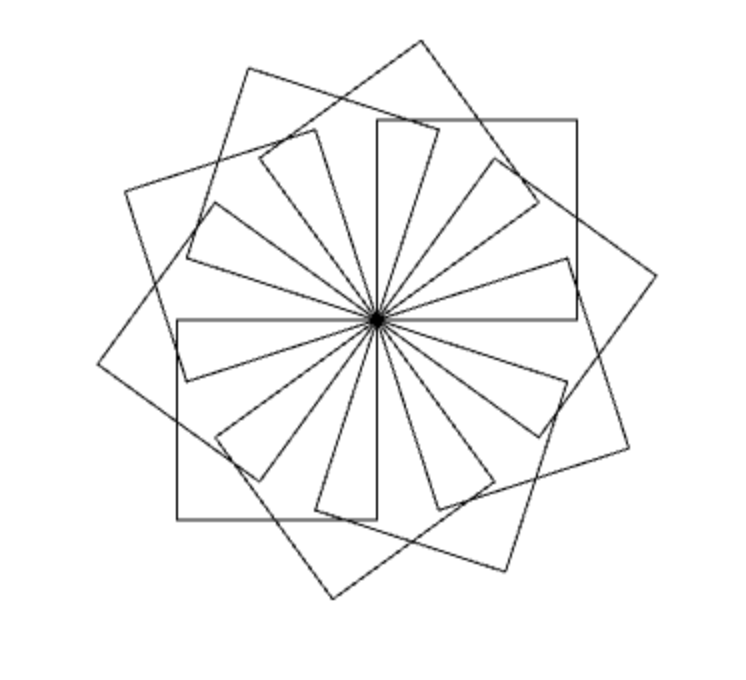
\includegraphics[width=0.6\columnwidth]{GrundlagenInfo/00_Programmieren/Figures/viereck_blume}
\end{figure}
\begin{itemize}
\item \textbf{Modularität}: Zerlegung des Programms in kleinere Stücke
\item \textbf{Übersichtlicher}!
\end{itemize}
\end{column}
\end{columns}
\end{frame}

\begin{frame}{Tipps}
\begin{itemize}
\item Turtle am Ende jedes Befehls wieder in gleiche Position bringen (Rotation, Ort)
\end{itemize}
\end{frame}

\begin{frame}[fragile]{Auftrag}
\begin{itemize}
\item \aufgabebox{Aufgaben 2.1 - 2.7}
\item \abgabebox{Abgabe auf Moodle: 2.7}
\item \aufgabebox{Aufgaben 2.8 - 2.18}
\item \abgabebox{Abgabe auf Moodle: 2.10}
\end{itemize}
\end{frame}